\section{Experiments}

In this section, we present empirical evaluation of our proposed work.
Specifically, the experiments aim to investigate the following three key questions.
\begin{itemize}
	\item \textbf{RQ1 (Overall performance).} Is the proposed \themodel able to improve non-pretraining baselines and outperform state-of-the-arts on molecular property prediction tasks?
	\item \textbf{RQ2 (Interpretation).} Are the learned attention weights of molecular featurizations on different downstream tasks consistent with chemical knowledge?
	\item \textbf{RQ3 (Ablation studies).} How do the representation aggregation module and the fine-tuning strategy affect the model performance?
\end{itemize}
In the following, we first summarize experimental setup and proceed to results and analysis.

\subsection{Experimental Configurations}

\paragraph{Datasets.}
We closely follow the experimental setup of GraphMVP \cite{Liu:2022vr} for fair comparison.
Specifically, we pretrain the model using the GEOM-Drugs dataset \cite{Axelrod:2022da} containing both 2D and 3D information.
For fine-tuning, we choose a variety datasets extracted from MoleculeNet \cite{Wu:2018dv}, ChEMBL \cite{Gaulton:2011ch}, and CEP \cite{Hachmann:2011ce}, that cover a wide range of applications, including physiological, biological, and pharmaceutical tasks, and QM9 \cite{Ramakrishnan:2014ij} that focuses on quantum property prediction.
These downstream tasks include 8 binary classification and 12 regression tasks.
For those datasets for fine-tuning, we follow OGB \cite{Hu:2020wv} that uses scaffolds to split training/test/validation subsets with a split ratio of 80\%/10\%/10\%.
For detailed description, we refer readers of interest to \cref{supp:dataset}.

\paragraph{Baselines.}
For comprehensive comparison, we select the following two groups of SSL methods as primary baselines in our experiments.
\begin{itemize}
	\item Generic graph SSL models: GraphSAGE \cite{Hamilton:2017tp}, InfoGraph \cite{Sun:2020vi}, GPT-GNN \cite{Hu:2020vh}, AttrMask, ContextPred \cite{Hu:2020uz}, GraphLoG \cite{Xu:2021tv}, GraphCL \cite{You:2020ut}, JOAO \cite{You:2021wl}, and GraphMAE \cite{Hou:2022jl}.
	\item Molecular SSL models: GROVER-Contextual (GROVER-C), GROVER-Motif (GROVER-M) \cite{Rong:2020vk}, and GraphMVP\footnote{In our experiments, we do not include its two variants GraphMVP-G and GraphMVP-C since they are essentially two ensemble models that combine AttrMask and ContextPred \cite{Hu:2020uz} respectively.} \cite{Liu:2022vr}.
\end{itemize}
In the pretraining stage, all the above SSL approaches are trained on the same dataset based on GEOM-Drugs.
We also report performance with a randomly initialized model as the non-pretraining baseline.
To ensure the performance is comparable with existing work, we report all baseline performance from previously published results \cite{Liu:2022vr,Hou:2022jl}.

\paragraph{Implementation details.}
\label{sec:implementation}

In the GEOM-Drugs dataset, since the original full set is too large (containing 317K molecules with over 9M conformations), we randomly select 50K molecules as the pretraining dataset.
For each molecule, we select to use its top-5 conformers of the lowest energy in virtue of their sufficient geometry information.
Since molecules in the fine-tuning datasets do not have 3D information available, we use ETKDG \cite{Riniker:2015bi} in RDkit \cite{Landrum:2022rd} to compute molecular conformations.
For both pretraining and fine-tuning datasets, we use RDkit to generate 1024-bit molecular fingerprints with radius $R=2$, which is roughly equivalent to the ECFP4 scheme \cite{Rogers:2010fp}.
We would like to emphasis that all dataset preprocessing and graph encoder architectures are kept in line with GraphMVP \cite{Liu:2022vr} to ensure fair comparison.
Readers of interest may refer to \cref{supp:implementation} for implementation details regarding software/hardware platforms, model training, and hyperparameter specifications.

\paragraph{Evaluation protocols.}
For classification tasks, we report the performance in terms of the Area Under the ROC-Curve (ROC-AUC), where higher values indicate better performance.
For quantum property and other non-quantum regression tasks, we measure the performance in Mean Absolute Error (MAE) and Root Mean Squared Error (RMSE) respectively, where lower values are better.
We repeat every experiment on three seeds with scaffold splitting and report the averaged performance with standard deviation, following previous work \cite{Liu:2022vr}.

\begin{table}
	\centering
	\caption{Results for eight molecule property prediction tasks in terms of ROC-AUC (\%, \(\uparrow\)). We highlight the best- and the second-best performing results in \textbf{boldface} and \underline{underlined}, respectively.}
	\label{tab:classification}
	\begin{tabular}{lccccccccc}
    \toprule
    Pretraining & BBBP & Tox21 & ToxCast & SIDER & ClinTox & MUV & HIV & BACE & Avg. \\
    \midrule
    --- & 71.0{\tiny±0.5} & \underline{75.9{\tiny±0.3}} & \underline{64.7{\tiny±2.3}} & 57.7{\tiny±3.1} & 71.5{\tiny±5.3} & \underline{77.7{\tiny±1.0}} & 75.9{\tiny±0.7} & 71.5{\tiny±2.7} & 70.63 \\
    \midrule
    GraphSAGE & 64.5{\tiny±3.1} & 74.5{\tiny±0.4} & 60.8{\tiny±0.5} & 56.7{\tiny±0.1} & 55.8{\tiny±6.2} & 73.3{\tiny±1.6} & 75.1{\tiny±0.8} & 64.6{\tiny±4.7} & 65.64 \\
    AttrMask & 70.2{\tiny±0.5} & 74.2{\tiny±0.8} & 62.5{\tiny±0.4} & 60.4{\tiny±0.6} & 68.6{\tiny±9.6} & 73.9{\tiny±1.3} & 74.3{\tiny±1.3} & 77.2{\tiny±1.4} & 70.16 \\
    GPT-GNN & 64.5{\tiny±1.1} & 75.3{\tiny±0.5} & 62.2{\tiny±0.1} & 57.5{\tiny±4.2} & 57.8{\tiny±3.1} & 76.1{\tiny±2.3} & 75.1{\tiny±0.2} & 77.6{\tiny±0.5} & 68.27 \\
    InfoGraph & 69.2{\tiny±0.8} & 73.0{\tiny±0.7} & 62.0{\tiny±0.3} & 59.2{\tiny±0.2} & 75.1{\tiny±5.0} & 74.0{\tiny±1.5} & 74.5{\tiny±1.8} & 73.9{\tiny±2.5} & 70.10 \\
    ContextPred & \underline{71.2{\tiny±0.9}} & 73.3{\tiny±0.5} & 62.8{\tiny±0.3} & 59.3{\tiny±1.4} & 73.7{\tiny±4.0} & 72.5{\tiny±2.2} & 75.8{\tiny±1.1} & 78.6{\tiny±1.4} & 70.89 \\
    GraphLoG & 67.8{\tiny±1.7} & 73.0{\tiny±0.3} & 62.2{\tiny±0.4} & 57.4{\tiny±2.3} & 62.0{\tiny±1.8} & 73.1{\tiny±1.7} & 73.4{\tiny±0.6} & 78.8{\tiny±0.7} & 68.47 \\
    GROVER-C & 70.3{\tiny±1.6} & 75.2{\tiny±0.3} & 62.6{\tiny±0.3} & 58.4{\tiny±0.6} & 59.9{\tiny±8.2} & 72.3{\tiny±0.9} & 75.9{\tiny±0.9} & 79.2{\tiny±0.3} & 69.21 \\
    GROVER-M & 66.4{\tiny±3.4} & 73.2{\tiny±0.8} & 62.6{\tiny±0.5} & 60.6{\tiny±1.1} & 77.8{\tiny±2.0} & 73.3{\tiny±2.0} & 73.8{\tiny±1.4} & 73.4{\tiny±4.0} & 70.14 \\
    GraphCL & 67.5{\tiny±3.3} & 75.0{\tiny±0.3} & 62.8{\tiny±0.2} & 60.1{\tiny±1.3} & 78.9{\tiny±4.2} & 77.1{\tiny±1.0} & 75.0{\tiny±0.4} & 68.7{\tiny±7.8} & 70.64 \\
    JOAO & 66.0{\tiny±0.6} & 74.4{\tiny±0.7} & 62.7{\tiny±0.6} & 60.7{\tiny±1.0} & 66.3{\tiny±3.9} & 77.0{\tiny±2.2} & 76.6{\tiny±0.5} & 72.9{\tiny±2.0} & 69.57 \\
    GraphMVP & 68.5{\tiny±0.2} & 74.5{\tiny±0.4} & 62.7{\tiny±0.1} & \textbf{62.3{\tiny±1.6}} & 79.0{\tiny±2.5} & 75.0{\tiny±1.4} & 74.8{\tiny±1.4} & 76.8{\tiny±1.1} & 71.69 \\
    GraphMAE & 70.9{\tiny±0.9} & 75.0{\tiny±0.4} & 64.1{\tiny±0.1} & 59.9{\tiny±0.5} & \underline{81.5{\tiny±2.8}} & 76.9{\tiny±2.6} & \underline{76.7{\tiny±0.9}} & \underline{81.4{\tiny±1.4}} & 73.31 \\
    \midrule
    \themodel &  \textbf{71.6{\tiny±1.0}} & \textbf{76.7{\tiny±0.4}} & \textbf{64.9{\tiny±0.8}} &
     \underline{61.2{\tiny±0.6}} & \textbf{81.6{\tiny±3.7}} & \textbf{78.5{\tiny±1.4}} & \textbf{78.3{\tiny±0.4}} & \textbf{82.6{\tiny±0.3}} & \textbf{74.41}\\
    \bottomrule
    \end{tabular}
\end{table}

\subsection{Main Results on Molecular Property Prediction}

The performance of molecular property prediction tasks is summarized in \cref{tab:classification}.
It can be found that our \themodel shows strong empirical performance across all eight low-data downstream datasets, delivering seven out of eight state-of-the-art results and acquiring a 1.1\% absolute improvement on average.
The outstanding results validate the superiority of our proposed model.

We make other observations as follows.
Firstly, \themodel obtains more accurate and stabler predictions compared to the randomly initialized baseline, indicating that our pretraining framework can transfer the knowledge from large, unannotated datasets to smaller downstream datasets without negative transfer.
Secondly, previous work has already achieved pretty high performance. For example, the current state-of-the-art GraphMVP only obtains a 0.8\% absolute improvement over its best baseline ContextPred in terms of average ROC-AUC. Our work pushes that boundary without extensive hyperparameter tuning, with an absolute improvement of up to 3.4\% over GraphMVP in terms of average ROC-AUC.
Lastly, it is worth mentioning that, the non-pretraining baseline even achieves better performance than some graph-based pretraining models. On some challenging datasets (e.g., Tox21, MUV, and ToxCast), it even achieves the second to best performance. This once more demonstrates the effectiveness of leveraging multiple featurization techniques.


\subsection{Interpretation and Analysis}


\begin{wrapfigure}{r}{0.4\textwidth}
	\setlength{\intextsep}{2pt}
	\centering
	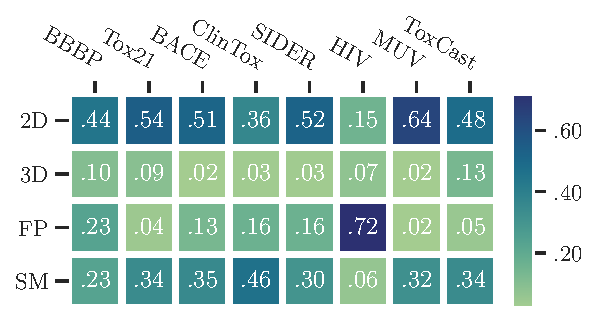
\includegraphics[width=\linewidth,bb=0 0 287 156]{figures/attention.pdf}
	\caption{Visualizing the learned attention weights on eight molecular property prediction datasets.}
	\label{fig:attention}
\end{wrapfigure}
In order to analyze the correlation between tasks and featurization techniques, we visualize the attention weights \(\bm\alpha\) learned on different downstream tasks in \cref{fig:attention}.
Note that most of the datasets in MoleculeNet \cite{Wu:2018dv} are ADMET property prediction tasks: chemical Absorption (A), Distribution (D), Metabolism (M), Excretion (E), and Toxicity (T), and we thus group the eight end tasks according to their prediction targets in the following analysis.

In general, we can interpret from the visualization that \emph{2D-based features are more significant than 3D-based features in the studied tasks}, which is well aligned with chemical knowledge. We provide detailed analysis as follows:
\begin{itemize}
\item In Tox21, ClinTox, SIDER, and ToxCast, we find that 2D graphs play the most important role. These four datasets are related to toxicity (or side effects). Although it is a very complex biological issue to explain, such properties can still be partially deduced from certain functional groups patterns contained in 2D graphs. Actually, medicinal chemists have developed such a database to provide them with necessary alerts of potential side effects in drug design \cite{Baell:2010ns}.
\item BBBP, which measures blood-brain barrier permeability, is mostly dominated by the following properties: liposolubility/water-solubility, molecular weight, and interaction between molecules and transporter proteins. Similarly, these properties can also be inferred from 2D topology, such as molecules with too many hydrogen bond acceptors/donors are unlikely to break the blood-brain barrier due to poor liposolubility \cite{Suckling:1986bb}.
\item On BACE and MUV we see 2D graphs and SMILES strings contribute most. These two datasets are about predicting protein-ligand binding activities, which are theoretically relevant to 3D conformations. However, it is still an open question that whether the conformation sampling methods can produce conformations that resemble bioactive conformations, which provide the key information for protein-ligand binding. Nevertheless, in each of these tasks, the target protein is fixed so that bioactivity can be partially deduced from 2D structures, which is supported by the success of fragment-based Quantitive Structure-Activity Relationship (QSAR) models \cite{Manoharan:2010qs}.
\item Due to the complicated pathogenetic mechanisms, it is hard to draw an explanation to why attention weights of fingerprints outweigh the other three features in the HIV task. Given that the HIV dataset is the largest one (over 40,000 molecules per task), one possible explanation of this phenomenon is that we use a high-dimensional fingerprint representations (1024 bits).
\end{itemize}

Concerning the difference between three 2D-based features (namely 2D topological graphs, fingerprints, and SMILES strings), we make the following findings, which we hope could serve as guidelines for future research on molecular representation learning:
\begin{itemize}
\item 2D graph representations can encode local information explicitly by resembling chemical structures. Besides, graph-based neural networks can capture long-range local chemical environment through message passing. For example, with molecular graphs, it is more convenient to identify which part of the molecule serves as a scaffold.
\item In principle, SMILES strings contain all 2D information of certain molecules, but with atoms and bonds represented in ASCII characters, neural networks may have difficulty in distilling semantic meanings of chemical structures in a numerical way.
\item Fingerprint representations are based on local structures and thus such features may be less effective in circumstances where long-range effects induced by topologically distant functional groups predominate, which accounts for relatively small attention weights of fingerprints in \cref{fig:attention}.
\end{itemize}


\subsection{More Experiments on Molecular Property Regression}

\begin{table}
    \centering
    \caption{Results for eight molecule quantum property regression tasks in terms of Mean Absolute Error (MAE, \(\downarrow\)). The highest performance is highlighted in \textbf{bold}.}
    \label{tab:quantum-regression}
    \begin{tabular}{cccccccccc}
    \toprule
    Target & \(\mu\) & \(\alpha\) & \(\epsilon_\text{HOMO}\) & \(\epsilon_\text{LUMO}\) & \(\epsilon_\text{gap}\) & \(U_0\) & \(U\) & \(\left<R^2\right>\) \\
    Unit & D & Bohr\textsuperscript{3} & meV & meV & meV & meV & meV & Bohr\textsuperscript{3}\\
    \midrule
    SchNet-NP & 0.4604 & 0.3251 & 95.9740 & 78.5870 & 136.4720 & 98.1240 & 100.1650 & 24.3277 \\
    \themodel-NP & 0.3767 & 0.2439 & 73.0625 & 69.8780 & 102.2332 & 77.4708 & 92.8562 & 17.5842 \\
    \midrule
    GraphMVP & 0.3726  & 0.4390  & 75.3750  & 72.3820  & 104.8370  & 278.8900  & 325.8021  & 22.6433  \\
    3D Infomax & 0.3644  & 0.4190  & 72.0558  & 67.6203  & 99.4032  & 207.2148  & 219.5415  & 20.3934 \\
    \themodel & \textbf{0.3618} & \textbf{0.2236} & \textbf{71.5120} & \textbf{58.5890} & \textbf{97.7440} & \textbf{64.3550} & \textbf{66.3958} & \textbf{15.5571} \\
    \bottomrule
    \end{tabular}
\end{table}

To demonstrate that the conformations generated by RDKit are helpful, we further conduct an experiment on quantum property regression on the QM9 dataset \cite{Ramakrishnan:2014ij}, where 3D conformations generated by RDKit are used for the fine-tuning datasets. This task is known to be closely related to 3D structures.
\cref{tab:quantum-regression} presents the performance comparison of MEMO with two non-pretraining (supervised) baselines SchNet and \themodel (denoted by SchNet-NP and \themodel-NP) and two state-of-the-art pretraining baselines GraphMVP \cite{Liu:2022vr} and 3D Infomax \cite{Stark:2021ug}.

It is seen that our \themodel model achieves the best performance on all datasets.
GraphMVP that consider only 2D structures during fine-tuning even result in negative transfer on some datasets. Our \themodel, on the contrary, achieves better performance than the supervised baseline, underscoring the value of leveraging 3D structures (as well as other sources of 2D information) during fine-tuning.

We also perform experiments on non-quantum property regression tasks. Our proposed \themodel also obtains promising improvements compared to the current state-of-the-art baselines. Please refer to \cref{supp:property-regression} for performance comparison and analysis.

\subsection{Ablation Studies}
\begin{figure}[b]
	\centering
	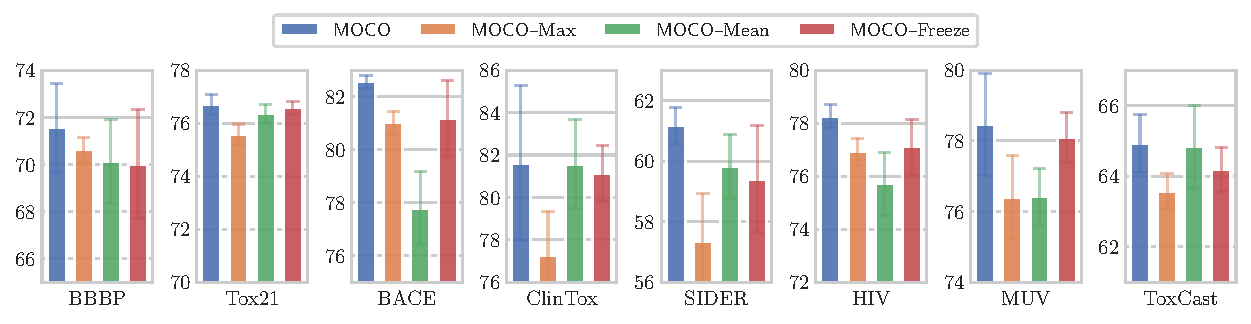
\includegraphics[width=\linewidth,bb=0 0 601 156]{figures/ablation.pdf}
	\caption{Ablation studies on representation aggregation and the fine-tuning strategy.}
	\label{fig:ablation}
\end{figure}

Finally, we conduct ablation studies on the representation aggregation module and the fine-tuning strategy.
We consider the following model variants for further inspection.
Except the modifications in specific modules, other implementations remain the same as previously described.
\begin{itemize}
	\item \textbf{\themodel --Max} removes the attention network in the representation aggregation module in \cref{eq:attention-aggregation} and simply uses max pooling to combine view embeddings.
	\item \textbf{\themodel --Mean} modifies representation aggregation by taking average over view embeddings.
	\item \textbf{\themodel --Freeze} does not fine-tune the representation aggregation module but instead uses the frozen weights of the pretrained model.
\end{itemize}

We report the performance of model variants in \cref{fig:ablation}.
It is seen that all three variants achieve downgraded performance, which empirically rationalizes the design choice of our molecular pretraining framework with complementary featurizations.
Specifically, the performance of \themodel --Max and \themodel --Mean without attention aggregation mechanisms of multiple featurizations is inferior to that of \themodel, demonstrating the necessity of adaptively combining information from multiple featurizations.
In addition, \themodel --Freeze occasionally obtains better performance than the two other variants, which indicates that our proposed attention network is able to select information from different views.
It does not, however, fine-tune the contribution of featurizations with downstream datasets, where the optimal combination might differ, resulting in performance deterioration.

Moreover, we conduct ablation studies on models that include only three view representations, where the results can be found in \cref{supp:more-ablation}. Results demonstrate the necessity of comprehensively leveraging four views in the proposed \themodel model.
